%=========================================================================
%  Bài tập Thống kê phi tham số — Chương 1
%  Biên dịch:  xelatex Chuong1_ECDF_BaiTap.tex   (chạy 2 lần)
%=========================================================================
\documentclass[12pt,a4paper]{article}

%--- Ngôn ngữ & font -----------------------------------------------------
\usepackage{fontspec}
\usepackage{polyglossia}
\setdefaultlanguage{vietnamese}
\setotherlanguage{english}
% Nạp theo tên file (TeX Gyre nằm trong texmf, không đăng ký với fontconfig)
\setmainfont{texgyretermes}[
  Extension=.otf, UprightFont=*-regular, BoldFont=*-bold,
  ItalicFont=*-italic, BoldItalicFont=*-bolditalic]
\setsansfont{texgyreheros}[
  Extension=.otf, UprightFont=*-regular, BoldFont=*-bold,
  ItalicFont=*-italic, BoldItalicFont=*-bolditalic]
% Menlo thiếu một số dấu tiếng Việt (ả, ỏ, ấ...) nên dùng TeX Gyre Cursor cho code
\setmonofont{texgyrecursor}[
  Extension=.otf, UprightFont=*-regular, BoldFont=*-bold,
  ItalicFont=*-italic, BoldItalicFont=*-bolditalic, Scale=0.86]

%--- Toán học ------------------------------------------------------------
\usepackage{amsmath}
\usepackage{unicode-math}
\setmathfont{texgyretermes-math.otf}
\allowdisplaybreaks

%--- Trình bày trang -----------------------------------------------------
\usepackage[a4paper,top=2.4cm,bottom=2.4cm,left=2.4cm,right=2.4cm]{geometry}
\usepackage{microtype}
\usepackage{parskip}
\usepackage{xcolor}
\usepackage{graphicx}
\usepackage{booktabs}
\usepackage{longtable}
\usepackage{array}
\usepackage{calc}
\usepackage{enumitem}
\setlist{topsep=3pt,itemsep=2pt,parsep=0pt}

\definecolor{accent}{HTML}{1F4E79}
\definecolor{accentlight}{HTML}{E8F0F8}
\definecolor{boxrule}{HTML}{9DB8D2}
\definecolor{codeframe}{HTML}{C9C9C9}
\definecolor{quotebar}{HTML}{B0B0B0}

%--- Đề mục --------------------------------------------------------------
\usepackage{titlesec}
\setcounter{secnumdepth}{-2}   % không đánh số tự động (số bài đã nằm trong tiêu đề)
\titleformat{\section}
  {\normalfont\Large\bfseries\color{accent}}{}{0pt}{}
  [\vspace{-6pt}{\color{boxrule}\rule{\linewidth}{0.8pt}}]
\titlespacing*{\section}{0pt}{18pt}{8pt}
\titleformat{\subsection}{\normalfont\large\bfseries\color{accent}}{}{0pt}{}
\titlespacing*{\subsection}{0pt}{12pt}{4pt}
\titleformat{\subsubsection}{\normalfont\normalsize\bfseries}{}{0pt}{}
\titlespacing*{\subsubsection}{0pt}{10pt}{3pt}

%--- Khung "Đề bài" và blockquote ---------------------------------------
\usepackage[skins,breakable]{tcolorbox}
\newtcolorbox{debai}{
  enhanced, breakable,
  colback=accentlight, colframe=accent,
  boxrule=0.7pt, arc=2pt,
  left=8pt, right=8pt, top=6pt, bottom=6pt,
  title=\textbf{Đề bài}, fonttitle=\normalsize
}
\newtcolorbox{ghichu}{
  enhanced, breakable, sharp corners,
  colback=white, colframe=white,
  borderline west={2.5pt}{0pt}{quotebar},
  boxrule=0pt, left=10pt, right=4pt, top=4pt, bottom=4pt
}
\renewenvironment{quote}{\begin{ghichu}}{\end{ghichu}}

%--- Khối code -----------------------------------------------------------
\usepackage{fvextra}
\DefineVerbatimEnvironment{verbatim}{Verbatim}
  {fontsize=\small, breaklines=true, breakanywhere=true,
   frame=single, rulecolor=\color{codeframe}, framesep=6pt,
   xleftmargin=0pt, samepage=false}

%--- Đầu/chân trang ------------------------------------------------------
\usepackage{fancyhdr}
\pagestyle{fancy}
\fancyhf{}
\fancyhead[L]{\small\color{accent}Thống kê phi tham số — Chương 1}
\fancyhead[R]{\small\thepage}
\renewcommand{\headrulewidth}{0.4pt}

%--- Liên kết ------------------------------------------------------------
\usepackage{hyperref}
\usepackage{xurl}
\hypersetup{
  colorlinks=true, linkcolor=accent, urlcolor=accent, citecolor=accent,
  pdftitle={Bài tập Thống kê phi tham số - Chương 1: Hàm phân phối tích lũy},
  pdfauthor={Cao học LT Thống kê Toán}
}
\usepackage{tikz}

\begin{document}

\begin{center}
  {\LARGE\bfseries\color{accent} Bài tập Thống kê phi tham số}\\[6pt]
  {\large Chương 1: Hàm mật độ xác suất tích lũy}\\[8pt]
  {\normalsize Lớp: Cao học LT Thống kê Toán}
\end{center}

\vspace{4pt}

\begin{ghichu}
\textbf{Ghi chú:} Kí hiệu \textbf{[W]} nghĩa là tham khảo sách \textit{All of Nonparametric Statistics} của Wasserman.

Mỗi bài gồm ba phần: \textbf{A. Motivation \& Ý nghĩa} (tại sao), \textbf{B. Chi tiết Toán học} (làm thế nào), \textbf{C. Ví dụ Thực tế \& Đa ngành} (dùng ở đâu).
\end{ghichu}

\vspace{6pt}

\section{\texorpdfstring{Bài 1. Khoảng tin cậy tiệm cận cho \(\sqrt{F(x_0)}\)}{Bài 1. Khoảng tin cậy tiệm cận cho \textbackslash sqrt\{F(x\_0)\}}}\label{buxe0i-1.-khoux1ea3ng-tin-cux1eady-tiux1ec7m-cux1eadn-cho-sqrtfx_0}

\begin{debai}

Xét \(X_1, \dots, X_n \overset{i.i.d}{\sim} F\), với \(F\) là một phân phối xác suất chưa biết, \(0 < F(x) < 1\) với \(x \in S \subset \mathbb{R}\), \(S\) là tập giá trị của \(X\). Dựa trên mẫu ngẫu nhiên này, hãy \textbf{xây dựng một khoảng tin cậy tiệm cận} với độ tin cậy \(100(1-\alpha)\%\) cho \(\sqrt{F(x_0)}\) với \(x_0\) cho trước thuộc \(S\).

\emph{Gợi ý: sử dụng hàm phân phối xác suất tích lũy thực nghiệm (ECDF) và phương pháp Delta (Delta-method).}

\end{debai}
\subsection*{Lời giải}

\subsubsection{A. Motivation \& Ý nghĩa (The ``Why'')}\label{a.-motivation-uxfd-nghux129a-the-why}

Trong thống kê phi tham số (Nonparametric Statistics), hàm phân phối tích lũy thực nghiệm (ECDF) \(\widehat{F}_n(x)\) là ước lượng không chệch và hội tụ hầu chắc chắn (Glivenko-Cantelli theorem) về \(F(x)\).

Khi cần suy diễn thống kê cho một hàm phi tuyến của phân phối \(\theta = g(F(x_0))\), cụ thể ở đây là phép biến đổi căn bậc hai \(g(t) = \sqrt{t}\), ta không thể áp dụng trực tiếp Định lý Giới hạn Trung tâm (CLT) dạng chuẩn. \textbf{Phương pháp Delta (Delta-method)} đóng vai trò xấp xỉ tuyến tính bậc nhất (Taylor expansion) của \(g\) quanh điểm \(F(x_0)\), chuyển phân phối tiệm cận của ECDF thành phân phối tiệm cận của \(\sqrt{\widehat{F}_n(x_0)}\) để xây dựng khoảng tin cậy tiệm cận (Asymptotic Confidence Interval).

\subsubsection{B. Chi tiết Toán học (The ``How'')}\label{b.-chi-tiux1ebft-touxe1n-hux1ecdc-the-how}

\emph{Bước 1: Phân phối tiệm cận của ECDF tại \(x_0\)}

\begin{itemize}

\item
  Định nghĩa biến chỉ thị \(Y_i = \mathbb{I}(X_i \le x_0)\) với \(i = 1, \dots, n\).
\item
  Các biến \(Y_i \overset{i.i.d}{\sim} \text{Bernoulli}(p)\), trong đó \(p = \mathbb{P}(X_i \le x_0) = F(x_0)\).
\item
  ECDF tại điểm cố định \(x_0\):
\end{itemize}

\[\widehat{F}_n(x_0) = \frac{1}{n} \sum_{i=1}^n \mathbb{I}(X_i \le x_0) = \bar{Y}\]

\begin{itemize}

\item
  Kỳ vọng và phương sai mẫu:
\end{itemize}

\[\mathbb{E}[\widehat{F}_n(x_0)] = F(x_0)\]

\[\text{Var}(\widehat{F}_n(x_0)) = \frac{F(x_0)(1 - F(x_0))}{n}\]

\begin{itemize}

\item
  Theo CLT:
\end{itemize}

\[\sqrt{n}\Big(\widehat{F}_n(x_0) - F(x_0)\Big) \xrightarrow{d} \mathcal{N}\Big(0, F(x_0)(1 - F(x_0))\Big)\]

\emph{Bước 2: Áp dụng Phương pháp Delta}

\begin{itemize}

\item
  Xét hàm \(g(t) = \sqrt{t}\) trên khoảng \((0, 1)\). Đạo hàm của \(g(t)\):
\end{itemize}

\[g'(t) = \frac{1}{2\sqrt{t}}\]

\begin{itemize}

\item
  Vì \(0 < F(x_0) < 1\), hàm \(g(t)\) khả vi liên tục tại \(t = F(x_0)\) và \(g'(F(x_0)) = \frac{1}{2\sqrt{F(x_0)}} \neq 0\).
\item
  Theo Delta-method, nếu \(\sqrt{n}(T_n - \theta) \xrightarrow{d} \mathcal{N}(0, \sigma^2)\) thì \(\sqrt{n}(g(T_n) - g(\theta)) \xrightarrow{d} \mathcal{N}(0, [g'(\theta)]^2 \sigma^2)\).
\item
  Tính phương sai tiệm cận:
\end{itemize}

\[\sigma_{\Delta}^2 = [g'(F(x_0))]^2 \cdot \text{Var}(Y_1) = \left(\frac{1}{2\sqrt{F(x_0)}}\right)^2 \cdot F(x_0)(1 - F(x_0)) = \frac{1}{4F(x_0)} \cdot F(x_0)(1 - F(x_0)) = \frac{1 - F(x_0)}{4}\]

\begin{itemize}

\item
  Ta thu được phân phối giới hạn:
\end{itemize}

\[\sqrt{n}\Big(\sqrt{\widehat{F}_n(x_0)} - \sqrt{F(x_0)}\Big) \xrightarrow{d} \mathcal{N}\left(0, \frac{1 - F(x_0)}{4}\right)\]

\emph{Bước 3: Ước lượng phương sai \& Bổ đề Slutsky}

\begin{itemize}

\item
  Tham số \(F(x_0)\) chưa biết được thay thế bằng ước lượng vững \(\widehat{F}_n(x_0)\).
\item
  Theo luật số lớn (WLLN) và Định lý Ánh xạ Liên tục (CMT):
\end{itemize}

\[\sqrt{\frac{1 - \widehat{F}_n(x_0)}{4}} \xrightarrow{P} \sqrt{\frac{1 - F(x_0)}{4}}\]

\begin{itemize}

\item
  Theo Định lý Slutsky, thống kê chuẩn hóa có phân phối tiệm cận chuẩn tắc:
\end{itemize}

\[\frac{\sqrt{\widehat{F}_n(x_0)} - \sqrt{F(x_0)}}{\sqrt{\dfrac{1 - \widehat{F}_n(x_0)}{4n}}} \xrightarrow{d} \mathcal{N}(0, 1)\]

\begin{itemize}

\item
  Sai số chuẩn ước lượng (Estimated Standard Error):
\end{itemize}

\[\widehat{\text{se}} = \frac{\sqrt{1 - \widehat{F}_n(x_0)}}{2\sqrt{n}}\]

\emph{Bước 4: Kết luận Khoảng tin cậy tiệm cận}

Khoảng tin cậy tiệm cận đối xứng \(100(1-\alpha)\%\) cho \(\sqrt{F(x_0)}\) là:

\[CI_{1-\alpha}\left(\sqrt{F(x_0)}\right) = \left[ \sqrt{\widehat{F}_n(x_0)} - z_{\alpha/2} \frac{\sqrt{1 - \widehat{F}_n(x_0)}}{2\sqrt{n}}, \; \sqrt{\widehat{F}_n(x_0)} + z_{\alpha/2} \frac{\sqrt{1 - \widehat{F}_n(x_0)}}{2\sqrt{n}} \right]\]

\emph{(Trong đó \(z_{\alpha/2}\) là giá trị tới hạn chuẩn tắc thỏa mãn \(\Phi(z_{\alpha/2}) = 1 - \alpha/2\). Nếu các mút vượt ngoài khoảng \([0, 1]\), ta cắt tỉa (truncate) về \([0, 1]\)).}

\subsubsection{C. Ví dụ Thực tế \& Đa ngành (The ``Where'')}\label{c.-vuxed-dux1ee5-thux1ef1c-tux1ebf-ux111a-nguxe0nh-the-where}

\begin{itemize}

\item
  \textbf{Data Drift \& Anomaly Detection (Security/IAM)}: Phép biến đổi căn bậc hai \(\sqrt{F(x)}\) thường xuất hiện khi tính toán \textbf{Khoảng cách Hellinger (Hellinger Distance)} hoặc hệ số \textbf{Bhattacharyya} để so sánh phân phối xác suất hành vi đăng nhập/truy cập tài nguyên của User giữa tập baseline và tập dữ liệu thời gian thực. Khoảng tin cậy cho \(\sqrt{F(x_0)}\) giúp thiết lập ngưỡng cảnh báo (dynamic thresholding) vững chắc khi phát hiện bất thường.
\item
  \textbf{Variance Stabilization}: Khi \(F(x_0) \to 0\) (sự kiện hiếm, ví dụ tỷ lệ rủi ro/fraud cực thấp), phương sai tiệm cận của \(\sqrt{\widehat{F}_n(x_0)}\) là \(\frac{1 - F(x_0)}{4n} \approx \frac{1}{4n}\), hầu như độc lập với giá trị \(F(x_0)\), giúp ổn định phương sai cho các mô hình suy diễn chuỗi thời gian hoặc streaming data.
\end{itemize}

\section{\texorpdfstring{Bài 2. Khoảng tin cậy Hoeffding cho tỷ lệ \(p\)}{Bài 2. Khoảng tin cậy Hoeffding cho tỷ lệ p}}\label{buxe0i-2.-khoux1ea3ng-tin-cux1eady-hoeffding-cho-tux1ef7-lux1ec7-p}

\begin{debai}

Xét \(X_1, \dots, X_n \overset{i.i.d}{\sim} \mathcal{B}(p)\). Với bất kỳ \(\epsilon > 0\), ta có

\[\mathbb{P}\big(\vert{}\bar{X} - p\vert{} > \epsilon\big) \le 2 e^{-2n\epsilon^2}\]

với \(\bar{X} = (1/n)\sum_{i=1}^n X_i\). Đây gọi là \textbf{bất đẳng thức Hoeffding} cho các biến ngẫu nhiên Bernoulli. Sử dụng bất đẳng thức này, hãy xây dựng một khoảng tin cậy \(100(1-\alpha)\%\) cho tỷ lệ \(p\). Viết 1 hàm trong \textbf{R} hoặc \textbf{Python} để tính khoảng tin cậy và tính \textbf{độ phủ (coverage)} thực tế của khoảng tin cậy tìm được.

\emph{Ghi chú trên đề (viết tay): \(\widehat{p} = \bar{X}\); mấu chốt là \textbf{chọn \(\epsilon = ?\)} --- đi từ \(\mathbb{P}(\vert{}\widehat{p}-p\vert{} \le \epsilon) \ge 1 - 2e^{-2n\epsilon^2} \to 1-\alpha\), suy ra \(\widehat{p} - \epsilon \le p \le \widehat{p} + \epsilon\).}

\end{debai}
\subsection*{Lời giải}

\subsubsection{A. Motivation \& Ý nghĩa (The ``Why'')}\label{a.-motivation-uxfd-nghux129a-the-why-1}

Trong thực tế xây dựng khoảng tin cậy, phương pháp cổ điển dựa trên Định lý Giới hạn Trung tâm (CLT/Wald Interval) chỉ đúng về mặt \textbf{tiệm cận} (\(n \to \infty\)). Khi kích thước mẫu \(n\) nhỏ hoặc hữu hạn, độ phủ thực tế (actual coverage probability) của khoảng tin cậy dạng Wald thường thấp hơn độ tin cậy danh định \(1 - \alpha\).

\textbf{Bất đẳng thức Hoeffding} cung cấp một chặn trên xác suất phi tham số, phi tiệm cận (\textbf{finite-sample distribution-free bound}). Khoảng tin cậy suy ra từ Hoeffding là một \textbf{khoảng tin cậy bảo thủ (conservative confidence interval)}: độ phủ thực tế luôn lớn hơn hoặc bằng \(1 - \alpha\) với mọi \(n \ge 1\), bất kể giá trị thực của tham số \(p\).

\subsubsection{B. Chi tiết Toán học (The ``How'')}\label{b.-chi-tiux1ebft-touxe1n-hux1ecdc-the-how-1}

\emph{Bước 1: Thiết lập Bất đẳng thức Hoeffding}

\begin{itemize}

\item
  Cho \(X_1, \dots, X_n \overset{i.i.d}{\sim} \text{Bernoulli}(p)\) với \(X_i \in [0, 1]\).
\item
  Ước lượng hợp lý cực đại cho \(p\) là trung bình mẫu:
\end{itemize}

\[\widehat{p} = \bar{X} = \frac{1}{n} \sum_{i=1}^n X_i\]

\begin{itemize}

\item
  Bất đẳng thức Hoeffding dạng hai phía (two-sided) cho các biến ngẫu nhiên độc lập bị chặn trong đoạn \([0, 1]\):
\end{itemize}

\[\mathbb{P}\big(\vert{}\widehat{p} - p\vert{} > \varepsilon\big) \le 2e^{-2n\varepsilon^2}, \quad \forall \varepsilon > 0\]

\emph{Bước 2: Tìm \(\varepsilon\) theo mức ý nghĩa \(\alpha\)}

\begin{itemize}

\item
  Chuyển sang biến cố bù:
\end{itemize}

\[\mathbb{P}\big(\vert{}\widehat{p} - p\vert{} \le \varepsilon\big) = 1 - \mathbb{P}\big(\vert{}\widehat{p} - p\vert{} > \varepsilon\big) \ge 1 - 2e^{-2n\varepsilon^2}\]

\begin{itemize}

\item
  Ta muốn độ tin cậy đạt ít nhất \(1 - \alpha\):
\end{itemize}

\[1 - 2e^{-2n\varepsilon^2} = 1 - \alpha \iff 2e^{-2n\varepsilon^2} = \alpha\]

\begin{itemize}

\item
  Giải phương trình tìm sai số \(\varepsilon\):
\end{itemize}

\[e^{-2n\varepsilon^2} = \frac{\alpha}{2} \iff -2n\varepsilon^2 = \ln\left(\frac{\alpha}{2}\right) = -\ln\left(\frac{2}{\alpha}\right)\]

\[\varepsilon_n = \sqrt{\frac{1}{2n} \ln\left(\frac{2}{\alpha}\right)}\]

\emph{Bước 3: Xây dựng Khoảng tin cậy}

\begin{itemize}

\item
  Biến cố \(\vert{}\widehat{p} - p\vert{} \le \varepsilon_n\) tương đương với:
\end{itemize}

\[\widehat{p} - \varepsilon_n \le p \le \widehat{p} + \varepsilon_n\]

\begin{itemize}

\item
  Vì tham số \(p \in [0, 1]\), ta cắt tỉa (truncate) các mút ra ngoài đoạn \([0, 1]\):
\end{itemize}

\[CI_{1-\alpha}(p) = \left[ \max\left(0, \, \widehat{p} - \sqrt{\frac{1}{2n}\ln\left(\frac{2}{\alpha}\right)}\right), \; \min\left(1, \, \widehat{p} + \sqrt{\frac{1}{2n}\ln\left(\frac{2}{\alpha}\right)}\right) \right]\]

\emph{Bước 4: Cài đặt code tính Khoảng tin cậy và Độ phủ (Coverage)}

\textbf{Phiên bản Python:}

\begin{verbatim}
import numpy as np

def hoeffding_ci_and_coverage(n, p, alpha=0.05, n_sim=10000, seed=42):
    """
    Tính khoảng tin cậy Hoeffding và empirical coverage qua mô phỏng Monte Carlo.
    """
    np.random.seed(seed)
    
    # 1. Tính epsilon từ bất đẳng thức Hoeffding
    eps = np.sqrt((1 / (2 * n)) * np.log(2 / alpha))
    
    # 2. Sinh n_sim mẫu Bernoulli(p), mỗi mẫu có kích thước n
    samples = np.random.binomial(n=1, p=p, size=(n_sim, n))
    p_hat = np.mean(samples, axis=1)
    
    # 3. Xây dựng cận dưới và cận trên
    lower_bound = np.clip(p_hat - eps, 0, 1)
    upper_bound = np.clip(p_hat + eps, 0, 1)
    
    # 4. Tính empirical coverage probability
    is_covered = (lower_bound <= p) & (p <= upper_bound)
    coverage = np.mean(is_covered)
    
    return {
        "epsilon": eps,
        "sample_ci_example": (lower_bound[0], upper_bound[0]),
        "nominal_confidence": 1 - alpha,
        "empirical_coverage": coverage
    }

# Chạy thử nghiệm với n = 100, p = 0.3, alpha = 0.05
res = hoeffding_ci_and_coverage(n=100, p=0.3, alpha=0.05)
print(f"Epsilon: {res['epsilon']:.4f}")
print(f"Ví dụ 1 CI: [{res['sample_ci_example'][0]:.4f}, {res['sample_ci_example'][1]:.4f}]")
print(f"Nominal Confidence: {res['nominal_confidence']:.2%}")
print(f"Empirical Coverage: {res['empirical_coverage']:.4%}")
\end{verbatim}

\textbf{Phiên bản R (tương đương):}

\begin{verbatim}
hoeffding_coverage <- function(n, p, alpha = 0.05, n_sim = 10000, seed = 42) {
  set.seed(seed)
  
  # Sai số Hoeffding
  eps <- sqrt((1 / (2 * n)) * log(2 / alpha))
  
  # Sinh dữ liệu mẫu & tính p_hat
  samples <- matrix(rbinom(n * n_sim, size = 1, prob = p), nrow = n_sim, ncol = n)
  p_hat <- rowMeans(samples)
  
  # Cận dưới và cận trên
  lower <- pmax(0, p_hat - eps)
  upper <- pmin(1, p_hat + eps)
  
  # Độ phủ thực tế
  coverage <- mean((lower <= p) & (p <= upper))
  
  return(list(
    epsilon = eps,
    example_CI = c(lower[1], upper[1]),
    nominal_confidence = 1 - alpha,
    empirical_coverage = coverage
  ))
}

# Chạy thử nghiệm
res_R <- hoeffding_coverage(n = 100, p = 0.3, alpha = 0.05)
print(res_R)
\end{verbatim}

\emph{Kết quả chạy thực tế (Python, \texttt{n\_sim\ =\ 10000}, \(\alpha = 0.05\), so sánh với khoảng Wald cổ điển):}

\begin{longtable}[]{@{}
  >{\raggedright\arraybackslash}p{(\linewidth - 10\tabcolsep) * \real{0.1667}}
  >{\raggedright\arraybackslash}p{(\linewidth - 10\tabcolsep) * \real{0.1667}}
  >{\raggedright\arraybackslash}p{(\linewidth - 10\tabcolsep) * \real{0.1667}}
  >{\raggedright\arraybackslash}p{(\linewidth - 10\tabcolsep) * \real{0.1667}}
  >{\raggedright\arraybackslash}p{(\linewidth - 10\tabcolsep) * \real{0.1667}}
  >{\raggedright\arraybackslash}p{(\linewidth - 10\tabcolsep) * \real{0.1667}}@{}}
\toprule\noalign{}
\begin{minipage}[b]{\linewidth}\raggedright
\(n\)
\end{minipage} & \begin{minipage}[b]{\linewidth}\raggedright
\(p\)
\end{minipage} & \begin{minipage}[b]{\linewidth}\raggedright
\(\varepsilon_n\)
\end{minipage} & \begin{minipage}[b]{\linewidth}\raggedright
Bề rộng \(2\varepsilon_n\)
\end{minipage} & \begin{minipage}[b]{\linewidth}\raggedright
Coverage Hoeffding
\end{minipage} & \begin{minipage}[b]{\linewidth}\raggedright
Coverage Wald
\end{minipage} \\
\midrule\noalign{}
\endhead
\bottomrule\noalign{}
\endlastfoot
10 & 0.1 & 0.4295 & 0.8589 & 0.9998 & 0.6524 \\
10 & 0.5 & 0.4295 & 0.8589 & 0.9978 & 0.8876 \\
30 & 0.3 & 0.2480 & 0.4959 & 0.9976 & 0.9548 \\
50 & 0.1 & 0.1921 & 0.3841 & 0.9999 & 0.8788 \\
100 & 0.3 & 0.1358 & 0.2716 & 0.9967 & 0.9512 \\
500 & 0.3 & 0.0607 & 0.1215 & 0.9974 & 0.9502 \\
1000 & 0.5 & 0.0429 & 0.0859 & 0.9924 & 0.9449 \\
\end{longtable}

\textbf{Nhận xét từ output thật:}

\begin{itemize}

\item
  Độ phủ thực tế của khoảng Hoeffding luôn \(\ge 0.99 \gg 0.95\) ở mọi \((n, p)\) đã thử --- đúng như lý thuyết dự đoán, đây là khoảng \textbf{bảo thủ (conservative)}: đảm bảo \(\ge 1-\alpha\) nhưng ``trả giá'' bằng bề rộng lớn.
\item
  Cái giá đó rất rõ ở mẫu nhỏ: với \(n = 10\), bề rộng \(2\varepsilon_n \approx 0.86\) gần như phủ trọn \([0,1]\) nên khoảng gần như vô dụng về mặt thông tin, dù coverage đạt \(99.98\%\).
\item
  Ngược lại, khoảng Wald chỉ đạt \(0.65\) (khi \(n=10, p=0.1\)) và \(0.88\) (khi \(n=50, p=0.1\)) --- thấp hơn hẳn mức danh định \(95\%\), minh họa đúng hiện tượng under-coverage của xấp xỉ CLT khi \(n\) nhỏ hoặc \(p\) gần biên.
\item
  Khi \(n\) tăng, coverage Wald mới tiến dần về \(0.95\), còn Hoeffding vẫn giữ mức \(\approx 0.99\); bề rộng Hoeffding giảm theo tốc độ \(\mathcal{O}(1/\sqrt{n})\) đúng như công thức \(\varepsilon_n = \sqrt{\ln(2/\alpha)/(2n)}\).
\end{itemize}

\subsubsection{C. Ví dụ Thực tế \& Đa ngành (The ``Where'')}\label{c.-vuxed-dux1ee5-thux1ef1c-tux1ebf-ux111a-nguxe0nh-the-where-1}

\begin{itemize}

\item
  \textbf{Service Level Objectives \& Threat Rate Bounds (Security/IAM)}: Khi đánh giá tỷ lệ đăng nhập thất bại do tấn công Credential Stuffing hoặc tỷ lệ request bất thường trên Gateway (\(p\)), ta thường có lượng mẫu kiểm thử nhỏ trong các khung giờ thấp điểm. Khoảng tin cậy Hoeffding đảm bảo một chặn trên chắc chắn 100\% về mặt toán học (finite-sample bound) mà không cần giả định xấp xỉ phân phối chuẩn.
\item
  \textbf{PAC Learning (Probably Approximately Correct Learning)}: Nền tảng của lý thuyết học máy sử dụng cận Hoeffding để chứng minh sai số tổng quát hóa (generalization error) của mô hình phân loại: với xác suất ít nhất \(1 - \delta\), sai số thực tế không vượt quá sai số trên tập huấn luyện cộng thêm một lượng \(\mathcal{O}\left(\sqrt{\frac{\ln(1/\delta)}{n}}\right)\).
\end{itemize}

\section{\texorpdfstring{Bài 3. Phân phối giới hạn của \(\sqrt{\widehat{F}_n(x)}\)}{Bài 3. Phân phối giới hạn của \textbackslash sqrt\{\textbackslash widehat\{F\}\_n(x)\}}}\label{buxe0i-3.-phuxe2n-phux1ed1i-giux1edbi-hux1ea1n-cux1ee7a-sqrtwidehatf_nx}

\begin{debai}

Xét \(X_1, X_2, \dots, X_n \sim F\) và xét \(\widehat{F}_n(x)\) là hàm phân phối tích lũy thực nghiệm. Với \(x\) cố định, tìm \textbf{phân phối giới hạn} của \(\sqrt{\widehat{F}_n(x)}\).

\emph{HD: sử dụng phương pháp Delta với \(g(x) = \sqrt{x}\), xem {[}W, chương 1, trang 4{]}. Cách làm giống Bài 1.}

\end{debai}
\subsection*{Lời giải}

\subsubsection{A. Motivation \& Ý nghĩa (The ``Why'')}\label{a.-motivation-uxfd-nghux129a-the-why-2}

Bài toán này yêu cầu tìm \textbf{hành vi ngẫu nhiên tiệm cận (Asymptotic/Limiting Distribution)} của đại lượng \(\sqrt{\widehat{F}_n(x)}\) khi kích thước mẫu \(n \to \infty\).

Bản chất của bài toán:

\begin{itemize}

\item
  Định lý Giới hạn Trung tâm (CLT) chỉ cho ta biết phân phối giới hạn của chính hàm thực nghiệm \(\widehat{F}_n(x)\) (bản chất là một trung bình mẫu).
\item
  Tuy nhiên, trong nhiều bài toán thống kê và Machine Learning, ta cần làm việc với các hàm phi tuyến \(g(\cdot)\) của phân phối (ví dụ như căn bậc hai \(\sqrt{\cdot}\) trong việc tính khoảng cách Hellinger hoặc ổn định phương sai).
\item
  Phương pháp Delta là công cụ vi phân xấp xỉ tuyến tính (Taylor bậc 1) giúp ``truyền'' phân phối chuẩn từ biến ban đầu sang hàm phi tuyến của nó.
\end{itemize}

\subsubsection{B. Chi tiết Toán học (The ``How'')}\label{b.-chi-tiux1ebft-touxe1n-hux1ecdc-the-how-2}

\emph{Bước 1: Phân phối tiệm cận gốc của ECDF theo CLT}

\begin{itemize}

\item
  Với điểm \(x\) cố định, đặt biến chỉ thị \(Y_i = \mathbb{I}(X_i \le x)\). Khi đó \(Y_1, \dots, Y_n \overset{i.i.d}{\sim} \text{Bernoulli}(F(x))\).
\item
  ECDF chính là trung bình mẫu:
\end{itemize}

\[\widehat{F}_n(x) = \frac{1}{n}\sum_{i=1}^n Y_i\]

\begin{itemize}

\item
  Theo Định lý Giới hạn Trung tâm (CLT):
\end{itemize}

\[\sqrt{n}\Big(\widehat{F}_n(x) - F(x)\Big) \xrightarrow{d} \mathcal{N}\Big(0, \sigma^2\Big)\]

trong đó phương sai gốc là:

\[\sigma^2 = \text{Var}(Y_i) = F(x)(1 - F(x))\]

\emph{Bước 2: Áp dụng Phương pháp Delta (Delta-Method)}

\begin{itemize}

\item
  Giả sử \(0 < F(x) < 1\).
\item
  Xét hàm chuyển đổi phi tuyến: \(g(t) = \sqrt{t} = t^{1/2}\).
\item
  Tính đạo hàm bậc nhất tại điểm \(t = F(x)\):
\end{itemize}

\[g'(t) = \frac{1}{2\sqrt{t}} \implies g'(F(x)) = \frac{1}{2\sqrt{F(x)}}\]

\begin{itemize}

\item
  Phương pháp Delta phát biểu: Nếu \(\sqrt{n}(T_n - \theta) \xrightarrow{d} \mathcal{N}(0, \sigma^2)\) và \(g'(\theta) \neq 0\), thì:
\end{itemize}

\[\sqrt{n}\Big(g(T_n) - g(\theta)\Big) \xrightarrow{d} \mathcal{N}\Big(0, [g'(\theta)]^2 \sigma^2\Big)\]

\emph{Bước 3: Tính phương sai tiệm cận mới}

\begin{itemize}

\item
  Thay \(g'(F(x))\) và \(\sigma^2\) vào công thức phương sai tiệm cận \(\sigma_{\Delta}^2\):
\end{itemize}

\[\sigma_{\Delta}^2 = [g'(F(x))]^2 \cdot \sigma^2 = \left(\frac{1}{2\sqrt{F(x)}}\right)^2 \cdot F(x)(1 - F(x))\]

\[\sigma_{\Delta}^2 = \frac{1}{4F(x)} \cdot F(x)(1 - F(x)) = \frac{1 - F(x)}{4}\]

\emph{Bước 4: Kết luận Phân phối giới hạn}

Phân phối giới hạn chuẩn hóa của \(\sqrt{\widehat{F}_n(x)}\) là:

\[\sqrt{n}\Big(\sqrt{\widehat{F}_n(x)} - \sqrt{F(x)}\Big) \xrightarrow{d} \mathcal{N}\left(0, \frac{1 - F(x)}{4}\right)\]

Hoặc viết dưới dạng xấp xỉ thực hành cho mẫu lớn:

\[\sqrt{\widehat{F}_n(x)} \underset{\text{approx}}{\sim} \mathcal{N}\left(\sqrt{F(x)}, \, \frac{1 - F(x)}{4n}\right)\]

\subsubsection{C. Ví dụ Thực tế \& Đa ngành (The ``Where'')}\label{c.-vuxed-dux1ee5-thux1ef1c-tux1ebf-ux111a-nguxe0nh-the-where-2}

\begin{itemize}

\item
  \textbf{Variance Stabilizing Transformation (Biến đổi ổn định phương sai)}: Phương sai ban đầu của \(\widehat{F}_n(x)\) là \(\frac{F(x)(1-F(x))}{n}\) (phụ thuộc phức tạp vào cả \(F(x)\) và \(1-F(x)\)). Khi áp dụng phép biến đổi căn bậc hai, phương sai tiệm cận trở thành \(\frac{1 - F(x)}{4n}\). Phép biến đổi này giúp đơn giản hóa phân phối, làm giảm sự phụ thuộc của phương sai vào giá trị trung bình ở vùng xác suất nhỏ.
\item
  \textbf{Goodness-of-Fit Testing (Kiểm định độ phù hợp mô hình)}: Phân phối giới hạn này là nền tảng để xây dựng thống kê kiểm định phi tham số dạng Freeman-Tukey hoặc khoảng cách Hellinger nhằm so sánh phân phối lý thuyết \(F_0\) với dữ liệu quan sát thực nghiệm \(\widehat{F}_n\) mà không lo ngại sự bùng nổ phương sai ở vùng đuôi dữ liệu.
\end{itemize}

\section{Bài 4. Hiệp phương sai của ECDF tại hai điểm}\label{buxe0i-4.-hiux1ec7p-phux1b0ux1a1ng-sai-cux1ee7a-ecdf-tux1ea1i-hai-ux111iux1ec3m}

\begin{debai}

Xét \(x\) và \(y\) là hai điểm phân biệt. Tìm \(\text{Cov}\left(\widehat{F}_n(x), \widehat{F}_n(y)\right)\).

\end{debai}
\subsection*{Lời giải}

\subsubsection{A. Motivation \& Ý nghĩa (The ``Why'')}\label{a.-motivation-uxfd-nghux129a-the-why-3}

Khi nghiên cứu hàm phân phối thực nghiệm \(\widehat{F}_n(x)\), ta không chỉ xem xét nó như một biến ngẫu nhiên đơn lẻ tại một điểm \(x\) cố định, mà là một \textbf{quá trình ngẫu nhiên (Empirical Process)} \(\left\{ \widehat{F}_n(x) : x \in \mathbb{R} \right\}\).

Việc tính hiệp phương sai \(\text{Cov}\big(\widehat{F}_n(x), \widehat{F}_n(y)\big)\) cho ta biết:

\begin{itemize}

\item
  Mức độ tương quan phụ thuộc giữa hai điểm \(x\) và \(y\) trên trục số.
\item
  Cấu trúc ma trận hiệp phương sai của phân phối chuẩn nhiều chiều tiệm cận \(\left(\widehat{F}_n(x_1), \dots, \widehat{F}_n(x_k)\right)^T\).
\item
  Nền tảng cấu trúc hàm tự hiệp phương sai (autocovariance function) dẫn tới quá trình \textbf{Cầu Brownian (Brownian Bridge)} trong Định lý Donsker (Donsker's Theorem) -- cốt lõi của các kiểm định phi tham số dạng Kolmogorov-Smirnov.
\end{itemize}

\subsubsection{B. Chi tiết Toán học (The ``How'')}\label{b.-chi-tiux1ebft-touxe1n-hux1ecdc-the-how-3}

\emph{Bước 1: Biểu diễn ECDF qua biến chỉ thị (Indicator Variables)}

\begin{itemize}

\item
  Đặt các biến chỉ thị:
\end{itemize}

\[I_i(x) = \mathbb{I}(X_i \le x) \quad \text{và} \quad I_j(y) = \mathbb{I}(X_j \le y)\]

\begin{itemize}

\item
  Khi đó:
\end{itemize}

\[\widehat{F}_n(x) = \frac{1}{n} \sum_{i=1}^n I_i(x), \qquad \widehat{F}_n(y) = \frac{1}{n} \sum_{j=1}^n I_j(y)\]

\emph{Bước 2: Phân rã Hiệp phương sai (Bilinear Property)}

\begin{itemize}

\item
  Sử dụng tính chất tuyến tính kép của hiệp phương sai:
\end{itemize}

\[\text{Cov}\left(\widehat{F}_n(x), \widehat{F}_n(y)\right) = \text{Cov}\left(\frac{1}{n}\sum_{i=1}^n I_i(x), \; \frac{1}{n}\sum_{j=1}^n I_j(y)\right) = \frac{1}{n^2} \sum_{i=1}^n \sum_{j=1}^n \text{Cov}\big(I_i(x), I_j(y)\big)\]

\begin{itemize}

\item
  Do \(X_1, X_2, \dots, X_n\) độc lập cùng phân phối (\(i.i.d\)):
\item
  Khi \(i \neq j\): \(I_i(x)\) và \(I_j(y)\) độc lập \(\implies \text{Cov}\big(I_i(x), I_j(y)\big) = 0\).
\item
  Khi \(i = j\): Ta chỉ còn tổng của \(n\) số hạng có chỉ số giống nhau:
\end{itemize}

\[\text{Cov}\left(\widehat{F}_n(x), \widehat{F}_n(y)\right) = \frac{1}{n^2} \sum_{i=1}^n \text{Cov}\big(I_i(x), I_i(y)\big) = \frac{1}{n} \text{Cov}\big(I_1(x), I_1(y)\big)\]

\emph{Bước 3: Tính hiệp phương sai của một cặp biến chỉ thị đơn lẻ}

\begin{itemize}

\item
  Theo định nghĩa hiệp phương sai:
\end{itemize}

\[\text{Cov}\big(I_1(x), I_1(y)\big) = \mathbb{E}\big[I_1(x) \cdot I_1(y)\big] - \mathbb{E}[I_1(x)] \cdot \mathbb{E}[I_1(y)]\]

\begin{itemize}

\item
  Tính từng thành phần:
\end{itemize}

\begin{enumerate}
\def\labelenumi{\arabic{enumi}.}

\item
  \(\mathbb{E}[I_1(x)] = \mathbb{P}(X_1 \le x) = F(x)\).
\item
  \(\mathbb{E}[I_1(y)] = \mathbb{P}(X_1 \le y) = F(y)\).
\item
  Tích hai biến chỉ thị:
\end{enumerate}

\[I_1(x) \cdot I_1(y) = \mathbb{I}(X_1 \le x \text{ và } X_1 \le y) = \mathbb{I}(X_1 \le \min(x, y))\]

Do đó:

\[\mathbb{E}\big[I_1(x) \cdot I_1(y)\big] = \mathbb{P}\big(X_1 \le \min(x, y)\big) = F\big(\min(x, y)\big)\]

\begin{itemize}

\item
  Thay vào công thức:
\end{itemize}

\[\text{Cov}\big(I_1(x), I_1(y)\big) = F\big(\min(x, y)\big) - F(x)F(y)\]

\emph{Bước 4: Kết luận}

Với hai điểm phân biệt \(x, y\):

\[\text{Cov}\left(\widehat{F}_n(x), \widehat{F}_n(y)\right) = \frac{F(\min(x, y)) - F(x)F(y)}{n}\]

\begin{quote}
\textbf{Kiểm tra tính nhất quán (Sanity Check):}
Nếu giả sử \(x = y\), công thức cho ra \(\frac{F(x) - F(x)^2}{n} = \frac{F(x)(1 - F(x))}{n} = \text{Var}\big(\widehat{F}_n(x)\big)\) (khớp hoàn toàn với phương sai của phân phối Bernoulli).
\end{quote}

\subsubsection{C. Ví dụ Thực tế \& Đa ngành (The ``Where'')}\label{c.-vuxed-dux1ee5-thux1ef1c-tux1ebf-ux111a-nguxe0nh-the-where-3}

\begin{itemize}

\item
  \textbf{Định lý Donsker \& Quá trình Brownian Bridge}: Quá trình ngẫu nhiên chuẩn hóa \(G_n(t) = \sqrt{n}\big(\widehat{F}_n(t) - F(t)\big)\) hội tụ theo luật sang quá trình Gauss \(G(t)\) có kỳ vọng 0 và hàm tự hiệp phương sai:
\end{itemize}

\[K(s, t) = F(\min(s, t)) - F(s)F(t)\]

Phép đổi biến xác suất \(u = F(t)\) chuyển quá trình này về đúng \textbf{Cầu Brownian} \(B(u)\) trên \([0, 1]\) với \(\text{Cov}(B(u), B(v)) = \min(u, v) - uv\). Đây chính là cơ sở toán học của kiểm định Kolmogorov-Smirnov dùng để phát hiện trôi dữ liệu (Data Drift).
* \textbf{Multi-threshold Monitoring (Hệ thống cảnh báo Security/Metrics)}: Khi thiết lập đồng thời nhiều ngưỡng cảnh báo \(x < y\) (ví dụ: ngưỡng \emph{Warning} \(x\) và ngưỡng \emph{Critical} \(y\) cho thời gian phản hồi hoặc kích thước payload), tỷ lệ vi phạm thực nghiệm \(\widehat{F}_n(x)\) và \(\widehat{F}_n(y)\) luôn có tương quan dương bằng \(\frac{F(x)(1 - F(y))}{n}\). Việc nắm rõ cấu trúc hiệp phương sai giúp tính toán chính xác xác suất kích hoạt báo động giả đồng thời trên cả hai ngưỡng.

\section{Bài 5. Phiếm hàm Lipschitz theo chuẩn sup \& Glivenko--Cantelli}\label{buxe0i-5.-phiux1ebfm-huxe0m-lipschitz-theo-chuux1ea9n-sup-glivenkocantelli}

\begin{debai}

Giả sử rằng

\[\vert{}T(F) - T(G)\vert{} \le C \Vert{}F - G\Vert{}_\infty \qquad (*)\]

với một hằng số \(0 < C < \infty\), trong đó \(\Vert{}F - G\Vert{}_\infty = \sup_x \vert{}F(x) - G(x)\vert{}\).

\textbf{(a)} Chứng minh rằng \(T(\widehat{F}_n) \xrightarrow{a.s.} T(F)\).

\textbf{(b)} Giả sử thêm rằng \(\vert{}X\vert{} \le M < \infty\). Hãy chứng minh rằng \(T(F) = \int x \, dF(x)\) thỏa mãn điều kiện \((*)\).

\emph{HD: sử dụng định lý Glivenko--Cantelli.}

\end{debai}
\subsection*{Lời giải}

\subsubsection{A. Motivation \& Ý nghĩa (The ``Why'')}\label{a.-motivation-uxfd-nghux129a-the-why-4}

Trong thống kê phi tham số, rất nhiều đại lượng ước lượng (như trung bình, phương sai, quantiles, trimmed mean) có thể biểu diễn dưới dạng một \textbf{phiếm hàm thống kê (Statistical Functional)} \(T(F)\).

Bài toán này khảo sát hai ý niệm nền tảng:

\begin{enumerate}
\def\labelenumi{\arabic{enumi}.}

\item
  \textbf{Tính trơn/Tính Lipschitz của phiếm hàm \(T(\cdot)\) theo chuẩn supremum \(\Vert{}\cdot\Vert{}_\infty\)}: Nếu một phiếm hàm \(T\) thỏa mãn tính chất Lipschitz đối với chuẩn sup, thì sự hội tụ đều của hàm phân phối sẽ trực tiếp kéo theo sự hội tụ mạnh (hầu chắc chắn - \emph{almost surely}) của ước lượng dạng cắm mẫu (plug-in estimator) \(T(\widehat{F}_n) \xrightarrow{a.s.} T(F)\).
\item
  \textbf{Cơ chế hoạt động của Định lý Glivenko-Cantelli (Định lý cơ bản của Thống kê)}: Cung cấp sự bảo đảm rằng \(\widehat{F}_n\) tiến đều về \(F\). Nhờ đó, ta dễ dàng chứng minh luật số lớn mạnh (SLLN) cho các đại lượng bị chặn thông qua cấu trúc giải tích của hàm tích lũy.
\end{enumerate}

\subsubsection{B. Chi tiết Toán học (The ``How'')}\label{b.-chi-tiux1ebft-touxe1n-hux1ecdc-the-how-4}

Bài toán gồm 2 phần chứng minh độc lập:

\paragraph{\texorpdfstring{Phần 1: Chứng minh \(T(\widehat{F}_n) \xrightarrow{a.s.} T(F)\)}{Phần 1: Chứng minh T(\textbackslash widehat\{F\}\_n) \textbackslash xrightarrow\{a.s.\} T(F)}}\label{phux1ea7n-1-chux1ee9ng-minh-twidehatf_n-xrightarrowa.s.-tf}

\emph{Bước 1: Áp dụng Định lý Glivenko-Cantelli}

\begin{itemize}

\item
  Theo Định lý Glivenko-Cantelli (định lý cơ bản của thống kê thực nghiệm), khi \(n \to \infty\), khoảng cách sup giữa ECDF \(\widehat{F}_n\) và hàm phân phối lý thuyết \(F\) hội tụ hầu chắc chắn về 0:
\end{itemize}

\[\Vert{}\widehat{F}_n - F\Vert{}_\infty = \sup_{x \in \mathbb{R}} \vert{}\widehat{F}_n(x) - F(x)\vert{} \xrightarrow{a.s.} 0\]

\emph{Bước 2: Sử dụng điều kiện Lipschitz (})*

\begin{itemize}

\item
  Thay \(G = \widehat{F}_n\) vào điều kiện \((*)\):
\end{itemize}

\[\vert{}T(\widehat{F}_n) - T(F)\vert{} \le C \Vert{}\widehat{F}_n - F\Vert{}_\infty\]

\begin{itemize}

\item
  Vì \(0 < C < \infty\) là một hằng số hữu hạn và \(\Vert{}\widehat{F}_n - F\Vert{}_\infty \xrightarrow{a.s.} 0\), ta có:
\end{itemize}

\[0 \le \lim_{n \to \infty} \vert{}T(\widehat{F}_n) - T(F)\vert{} \le C \cdot \lim_{n \to \infty} \Vert{}\widehat{F}_n - F\Vert{}_\infty = C \cdot 0 = 0 \quad (\text{hầu chắc chắn})\]

\begin{itemize}

\item
  Suy ra:
\end{itemize}

\[T(\widehat{F}_n) \xrightarrow{a.s.} T(F)\]

\paragraph{\texorpdfstring{Phần 2: Chứng minh \(T(F) = \int x \, dF(x)\) thỏa mãn điều kiện (*) khi \(\vert{}X\vert{} \le M < \infty\)}{Phần 2: Chứng minh T(F) = \textbackslash int x \textbackslash, dF(x) thỏa mãn điều kiện (*) khi \textbackslash vert\{\}X\textbackslash vert\{\} \textbackslash le M \textless{} \textbackslash infty}}\label{phux1ea7n-2-chux1ee9ng-minh-tf-int-x-dfx-thux1ecfa-muxe3n-ux111iux1ec1u-kiux1ec7n-khi-vertxvert-le-m-infty}

Giả thiết \(\vert{}X\vert{} \le M < \infty\) đồng nghĩa với việc phân phối xác suất của \(X\) được nâng đỡ hoàn toàn trên đoạn \([-M, M]\).
Do đó:

\begin{itemize}

\item
  \(F(x) = 0\) với mọi \(x < -M\)
\item
  \(F(x) = 1\) với mọi \(x \ge M\)
  \emph{(Tương tự với phân phối \(G\) bất kỳ cũng được hỗ trợ trên \([-M, M]\))}
\end{itemize}

\emph{Bước 1: Tích phân từng phần (Integration by Parts)}

\begin{itemize}

\item
  Xét tích phân Riemann-Stieltjes của kỳ vọng:
\end{itemize}

\[T(F) = \int_{-M}^M x \, dF(x)\]

\begin{itemize}

\item
  Áp dụng công thức tích phân từng phần: \(\int u\, dv = uv - \int v\, du\):
\end{itemize}

\[T(F) = \Big[ x F(x) \Big]_{-M}^{M} - \int_{-M}^M F(x) \, dx\]

\begin{itemize}

\item
  Thay cận tại \(M\) và \(-M\):
\end{itemize}

\[\Big[ x F(x) \Big]_{-M}^{M} = M \cdot F(M) - (-M) \cdot F(-M) = M \cdot 1 - (-M) \cdot 0 = M\]

\begin{itemize}

\item
  Do đó, ta biểu diễn được phiếm hàm kỳ vọng thuần túy qua diện tích dưới hàm \(F\):
\end{itemize}

\[T(F) = M - \int_{-M}^M F(x) \, dx\]

\emph{Bước 2: Thiết lập đánh giá sai phân \(\vert{}T(F) - T(G)\vert{}\)}

\begin{itemize}

\item
  Tương tự với phân phối \(G\):
\end{itemize}

\[T(G) = M - \int_{-M}^M G(x) \, dx\]

\begin{itemize}

\item
  Lấy hiệu hai phiếm hàm:
\end{itemize}

\[T(F) - T(G) = \left( M - \int_{-M}^M F(x) \, dx \right) - \left( M - \int_{-M}^M G(x) \, dx \right) = \int_{-M}^M \big(G(x) - F(x)\big) \, dx\]

\emph{Bước 3: Lấy trị tuyệt đối và đánh giá chặn trên}

\begin{itemize}

\item
  Dùng bất đẳng thức tích phân:
\end{itemize}

\[\vert{}T(F) - T(G)\vert{} = \left\vert{} \int_{-M}^M \big(F(x) - G(x)\big) \, dx \right\vert{} \le \int_{-M}^M \vert{}F(x) - G(x)\vert{} \, dx\]

\begin{itemize}

\item
  Với mọi \(x \in [-M, M]\), theo định nghĩa của chuẩn sup:
\end{itemize}

\[\vert{}F(x) - G(x)\vert{} \le \sup_{t \in \mathbb{R}} \vert{}F(t) - G(t)\vert{} = \Vert{}F - G\Vert{}_\infty\]

\begin{itemize}

\item
  Do đó:
\end{itemize}

\[\vert{}T(F) - T(G)\vert{} \le \int_{-M}^M \Vert{}F - G\Vert{}_\infty \, dx = \Vert{}F - G\Vert{}_\infty \int_{-M}^M 1 \, dx = 2M \Vert{}F - G\Vert{}_\infty\]

\emph{Bước 4: Kết luận}

\begin{itemize}

\item
  Chọn hằng số \(C = 2M < \infty\), ta có:
\end{itemize}

\[\vert{}T(F) - T(G)\vert{} \le C \Vert{}F - G\Vert{}_\infty\]

\begin{itemize}

\item
  Vậy phiếm hàm \(T(F) = \int x \, dF(x)\) thỏa mãn trọn vẹn điều kiện \((*)\).
\end{itemize}

\subsubsection{C. Ví dụ Thực tế \& Đa ngành (The ``Where'')}\label{c.-vuxed-dux1ee5-thux1ef1c-tux1ebf-ux111a-nguxe0nh-the-where-4}

\begin{itemize}

\item
  \textbf{Robust Statistics \& Influence Functions (Thống kê Vững)}: Tính chất Lipschitz đối với chuẩn \(\Vert{}\cdot\Vert{}_\infty\) liên quan mật thiết đến tính ổn định của ước lượng thống kê trước nhiễu hoặc dữ liệu dị biệt (outliers/data poisoning). Nếu một thống kê \(T(F)\) có tính Lipschitz theo \(\Vert{}\cdot\Vert{}_\infty\), giá trị ước lượng sẽ không bị bùng nổ khi dữ liệu bị chèn một tỷ lệ phần trăm nhỏ các bản ghi tấn công độc hại.
\item
  \textbf{Bounded Reward in Reinforcement Learning \& Security}: Trong các bài toán học tăng cường (RL) hoặc tính toán tổn thất rủi ro gian lận tài chính mà Reward/Loss bị chặn trong khoảng \([-M, M]\), việc xấp xỉ hàm phân phối xác suất môi trường \(F\) bằng mô hình thực nghiệm \(\widehat{F}_n\) đảm bảo giá trị kỳ vọng tích lũy hội tụ đều hầu chắc chắn với tốc độ co được kiểm soát bởi \(2M\).
\end{itemize}

\section{Bài 6. Tính và phác họa ECDF}\label{buxe0i-6.-tuxednh-vuxe0-phuxe1c-hux1ecda-ecdf}

\begin{debai}

\textbf{Tính hàm phân phối thực nghiệm (ECDF):}

\textbf{(a)} Với mẫu số liệu \(\{2.3,\ 1.7,\ 4.1,\ 3.5,\ 2.3,\ 5.0\}\), hãy tính và phác họa hàm phân phối thực nghiệm (ECDF).

\textbf{(b)} Tính giá trị của ECDF tại \(x = 3.0\) và \(x = 4.5\).

\textbf{(c)} Xác định trung vị mẫu và phân vị thứ 75\% dựa vào ECDF.

\end{debai}
\subsection*{Lời giải}

\subsubsection{A. Motivation \& Ý nghĩa (The ``Why'')}\label{a.-motivation-uxfd-nghux129a-the-why-5}

Hàm phân phối thực nghiệm (ECDF - Empirical Cumulative Distribution Function) \(\widehat{F}_n(x)\) là hàm từng đoạn dạng bậc thang (step function) gán trọng số đều \(\frac{1}{n}\) cho mỗi quan sát trong mẫu.

\begin{itemize}

\item
  ECDF là ước lượng phi tham số (nonparametric) cho phân phối tích lũy lý thuyết \(F(x)\) mà không đòi hỏi bất kỳ giả định nào về dạng hàm phân phối (không cần giả định chuẩn, đều, mũ\ldots).
\item
  Các thống kê thứ tự (order statistics) và phân vị mẫu (quantiles/median) được định nghĩa trực tiếp từ hàm ngược suy rộng của ECDF: \(\widehat{F}_n^{-1}(p) = \inf \{x : \widehat{F}_n(x) \ge p\}\).
\end{itemize}

\subsubsection{B. Chi tiết Toán học (The ``How'')}\label{b.-chi-tiux1ebft-touxe1n-hux1ecdc-the-how-5}

Cho mẫu số liệu \(n = 6\): \(\{2.3, 1.7, 4.1, 3.5, 2.3, 5.0\}\).

\emph{Sắp xếp mẫu theo thứ tự tăng dần (Order Statistics):}

\[X_{(1)} = 1.7, \quad X_{(2)} = 2.3, \quad X_{(3)} = 2.3, \quad X_{(4)} = 3.5, \quad X_{(5)} = 4.1, \quad X_{(6)} = 5.0\]

\emph{(a) Tính và phác họa hàm phân phối thực nghiệm \(\widehat{F}_n(x)\)}

Công thức định nghĩa:

\[\widehat{F}_n(x) = \frac{1}{n} \sum_{i=1}^n \mathbb{I}(X_i \le x) = \frac{\text{Số quan sát } \le x}{6}\]

Xác định giá trị tại từng khoảng:

\begin{itemize}

\item
  Nếu \(x < 1.7\): không có điểm nào \(\implies \widehat{F}_n(x) = 0\).
\item
  Nếu \(1.7 \le x < 2.3\): có 1 điểm (\(1.7\)) \(\implies \widehat{F}_n(x) = \frac{1}{6} \approx 0.1667\).
\item
  Nếu \(2.3 \le x < 3.5\): có 3 điểm (\(1.7, 2.3, 2.3\)) do \(2.3\) lặp lại 2 lần \(\implies\) bước nhảy có độ cao \(\frac{2}{6}\), \(\widehat{F}_n(x) = \frac{3}{6} = 0.5\).
\item
  Nếu \(3.5 \le x < 4.1\): có 4 điểm (\(1.7, 2.3, 2.3, 3.5\)) \(\implies \widehat{F}_n(x) = \frac{4}{6} = \frac{2}{3} \approx 0.6667\).
\item
  Nếu \(4.1 \le x < 5.0\): có 5 điểm \(\implies \widehat{F}_n(x) = \frac{5}{6} \approx 0.8333\).
\item
  Nếu \(x \ge 5.0\): cả 6 điểm đều \(\le x\) \(\implies \widehat{F}_n(x) = \frac{6}{6} = 1.0\).
\end{itemize}

Tổng hợp biểu thức của \(\widehat{F}_n(x)\):

\[\widehat{F}_n(x) = \begin{cases}  0, & x < 1.7 \\  \frac{1}{6}, & 1.7 \le x < 2.3 \\  \frac{1}{2}, & 2.3 \le x < 3.5 \\  \frac{2}{3}, & 3.5 \le x < 4.1 \\  \frac{5}{6}, & 4.1 \le x < 5.0 \\  1, & x \ge 5.0  \end{cases}\]

\emph{Phác họa đồ thị bậc thang:}

\begin{center}
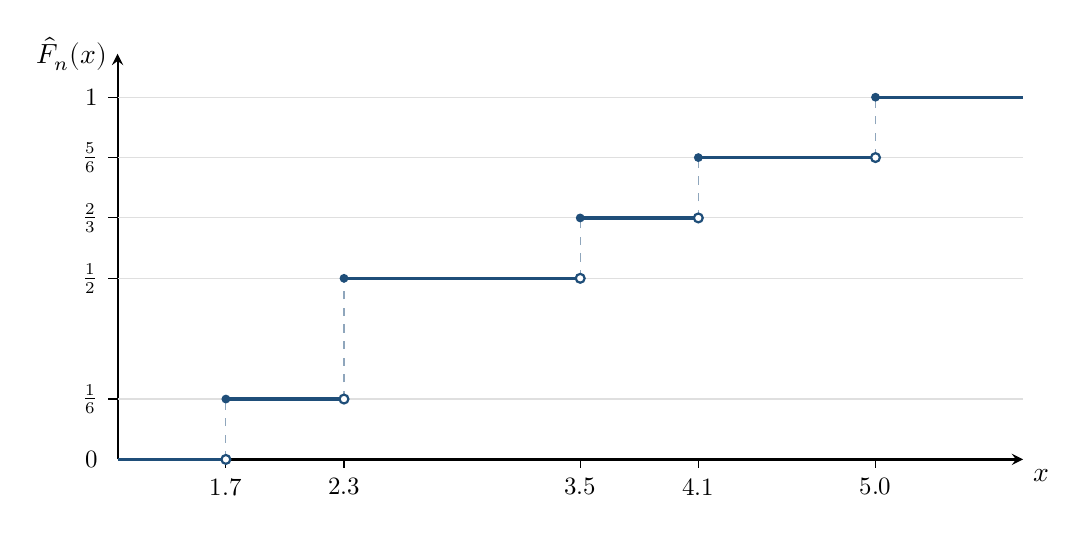
\begin{tikzpicture}[x=2.5cm, y=4.6cm, >=stealth]
  % trục
  \draw[->,thick] (1.15,0) -- (5.75,0) node[below right] {$x$};
  \draw[->,thick] (1.15,0) -- (1.15,1.12) node[left] {$\widehat{F}_n(x)$};
  % lưới ngang mờ
  \foreach \y/\lb in {0.16667/$\frac{1}{6}$, 0.5/$\frac{1}{2}$, 0.66667/$\frac{2}{3}$,
                      0.83333/$\frac{5}{6}$, 1/$1$}{
    \draw[gray!25] (1.15,\y) -- (5.75,\y);
    \draw (1.15,\y) -- (1.10,\y) node[left] {\small \lb};
  }
  \node[left] at (1.10,0) {\small $0$};
  % vạch trục hoành
  \foreach \x in {1.7, 2.3, 3.5, 4.1, 5.0}{
    \draw (\x,0) -- (\x,-0.025) node[below] {\small $\x$};
  }
  % các bậc thang
  \draw[very thick, accent] (1.15,0)       -- (1.7,0);
  \draw[very thick, accent] (1.7,0.16667)  -- (2.3,0.16667);
  \draw[very thick, accent] (2.3,0.5)      -- (3.5,0.5);
  \draw[very thick, accent] (3.5,0.66667)  -- (4.1,0.66667);
  \draw[very thick, accent] (4.1,0.83333)  -- (5.0,0.83333);
  \draw[very thick, accent] (5.0,1)        -- (5.75,1);
  % bước nhảy (nét đứt)
  \foreach \x/\a/\b in {1.7/0/0.16667, 2.3/0.16667/0.5, 3.5/0.5/0.66667,
                        4.1/0.66667/0.83333, 5.0/0.83333/1}{
    \draw[dashed, accent!50] (\x,\a) -- (\x,\b);
    \fill[accent] (\x,\b) circle (1.6pt);                       % điểm đóng
    \draw[accent, fill=white, thick] (\x,\a) circle (1.6pt);     % điểm mở
  }
\end{tikzpicture}
\end{center}

\emph{(Dấu \(\bullet\) biểu thị điểm đóng thuộc khoảng tại mút trái, dấu \(\circ\) biểu thị điểm mở tại mút phải do tính liên tục phải của CDF)}.

\emph{(b) Tính giá trị của ECDF tại \(x = 3.0\) và \(x = 4.5\)}

\begin{itemize}

\item
  \textbf{Tại \(x = 3.0\):}
  Vì \(2.3 \le 3.0 < 3.5\), các phần tử trong mẫu thỏa mãn \(X_i \le 3.0\) gồm \(\{1.7, 2.3, 2.3\}\) (3 phần tử).
\end{itemize}

\[\widehat{F}_n(3.0) = \frac{3}{6} = 0.5\]

\begin{itemize}

\item
  \textbf{Tại \(x = 4.5\):}
  Vì \(4.1 \le 4.5 < 5.0\), các phần tử thỏa mãn \(X_i \le 4.5\) gồm \(\{1.7, 2.3, 2.3, 3.5, 4.1\}\) (5 phần tử).
\end{itemize}

\[\widehat{F}_n(4.5) = \frac{5}{6} \approx 0.8333\]

\emph{(c) Xác định Trung vị mẫu (Sample Median) và Phân vị thứ 75\% (75th Percentile)}

Theo định nghĩa phân vị phi tham số chuẩn tắc \(\widehat{q}(p) = \widehat{F}_n^{-1}(p) = \inf \{x : \widehat{F}_n(x) \ge p\}\):

\begin{itemize}

\item
  \textbf{Trung vị mẫu (\(p = 0.5\)):}
  Ta tìm giá trị \(x\) nhỏ nhất sao cho \(\widehat{F}_n(x) \ge 0.5\).
  Nhìn vào bảng giá trị: \(\widehat{F}_n(x) = 0.5\) bắt đầu đạt được chính xác tại \(x = 2.3\).
\end{itemize}

\[\text{Sample Median} = 2.3\]

\emph{(Nếu áp dụng định nghĩa nội suy trung bình hai điểm giữa cho \(n=6\) chẵn: \(\frac{X_{(3)} + X_{(4)}}{2} = \frac{2.3 + 3.5}{2} = 2.9\). Tuy nhiên, theo định nghĩa trực tiếp từ ECDF Step Function, trung vị chuẩn là \(2.3\))}.
* \textbf{Phân vị thứ 75\% (\(p = 0.75\)):}
Ta tìm \(x\) nhỏ nhất sao cho \(\widehat{F}_n(x) \ge 0.75\).
* Tại khoảng \([3.5, 4.1)\), \(\widehat{F}_n(x) = \frac{4}{6} \approx 0.6667 < 0.75\).
* Tại điểm \(x = 4.1\), hàm nhảy lên \(\widehat{F}_n(4.1) = \frac{5}{6} \approx 0.8333 \ge 0.75\).

\[\text{75th Percentile } (\widehat{q}_{0.75}) = 4.1\]

\subsubsection{C. Ví dụ Thực tế \& Đa ngành (The ``Where'')}\label{c.-vuxed-dux1ee5-thux1ef1c-tux1ebf-ux111a-nguxe0nh-the-where-5}

\begin{itemize}

\item
  \textbf{SLA \& Latency Percentile Monitoring (DevOps / Network Security)}: Khi đo đạc độ trễ API (response time), ECDF được xây dựng trực tiếp trên các log request streaming. Các ngưỡng P50 (median) và P75 (hoặc P99) suy ra trực tiếp từ ECDF mà không cần giả định phân phối log-normal, giúp hệ thống phát hiện chính xác tình trạng suy thoái hiệu năng hệ thống.
\end{itemize}

\section{Bài 7. Kiểm định phù hợp Kolmogorov--Smirnov}\label{buxe0i-7.-kiux1ec3m-ux111ux1ecbnh-phuxf9-hux1ee3p-kolmogorovsmirnov}

\begin{debai}

\textbf{Kiểm định sự phù hợp (Goodness-of-Fit Test):}

\textbf{(a)} Sử dụng mẫu dữ liệu ở Bài 5, hãy kiểm định giả thuyết rằng dữ liệu tuân theo phân phối đều trên khoảng \([1, 5]\) bằng kiểm định Kolmogorov--Smirnov (K--S test).

\textbf{(b)} Tính thống kê kiểm định K--S và xấp xỉ giá trị p-value bằng phân phối tiệm cận.

\textbf{(c)} Diễn giải kết quả kiểm định ở mức ý nghĩa 5\%.

\begin{quote}
\emph{Lưu ý:} đề ghi ``mẫu dữ liệu ở Bài 5'', nhưng mẫu số liệu \(\{2.3, 1.7, 4.1, 3.5, 2.3, 5.0\}\) thực chất nằm ở \textbf{Bài 6}. Lời giải dưới đây dùng mẫu đó.
\end{quote}

\end{debai}
\subsection*{Lời giải}

\subsubsection{A. Motivation \& Ý nghĩa (The ``Why'')}\label{a.-motivation-uxfd-nghux129a-the-why-6}

Kiểm định Kolmogorov-Smirnov (K-S test) là một trong những phương pháp kiểm định độ phù hợp (Goodness-of-Fit) phi tham số kinh điển nhất.

\begin{itemize}

\item
  \textbf{Bản chất}: Thay vì nhóm dữ liệu thành các khoảng rời rạc (bins) như kiểm định Chi-bình phương (\(\chi^2\)), K-S test so sánh trực tiếp khoảng cách lớn nhất (chuẩn supremum \(\Vert{}\cdot\Vert{}_\infty\)) giữa hàm phân phối thực nghiệm \(\widehat{F}_n(x)\) và hàm phân phối lý thuyết \(F_0(x)\).
\item
  \textbf{Ưu điểm}: Phù hợp với các biến ngẫu nhiên liên tục, bảo toàn toàn bộ thông tin của từng điểm dữ liệu riêng lẻ và độc lập với phân phối lý thuyết được kiểm định (distribution-free under \(H_0\)).
\end{itemize}

\subsubsection{B. Chi tiết Toán học (The ``How'')}\label{b.-chi-tiux1ebft-touxe1n-hux1ecdc-the-how-6}

Cho mẫu số liệu \(n = 6\) (sắp xếp tăng dần):

\[X_{(1)} = 1.7, \quad X_{(2)} = 2.3, \quad X_{(3)} = 2.3, \quad X_{(4)} = 3.5, \quad X_{(5)} = 4.1, \quad X_{(6)} = 5.0\]

\emph{(a) Thiết lập bài toán kiểm định}

\begin{itemize}
\item
  \textbf{Giả thuyết}:
\item
  \(H_0\): Dữ liệu tuân theo phân phối đều trên khoảng \([1, 5]\), tức \(X \sim U[1, 5]\).
\item
  \(H_1\): Dữ liệu không tuân theo phân phối đều trên \([1, 5]\).
\item
  \textbf{Hàm phân phối tích lũy lý thuyết dưới \(H_0\)}:
\end{itemize}

\[F_0(x) = \begin{cases}    0, & x < 1 \\    \frac{x - 1}{5 - 1} = \frac{x - 1}{4}, & 1 \le x \le 5 \\    1, & x > 5    \end{cases}\]

\emph{(b) Tính thống kê kiểm định \(D_n\) và xấp xỉ p-value}

\emph{Bước 1: Tính các độ lệch tại từng điểm quan sát}
Thống kê K-S hai phía được định nghĩa bởi:

\[D_n = \sup_{x} \vert{}\widehat{F}_n(x) - F_0(x)\vert{} = \max_{1 \le i \le n} \left\{ \max\left( \left\vert{}\frac{i}{n} - F_0(X_{(i)})\right\vert{}, \; \left\vert{}F_0(X_{(i)}) - \frac{i-1}{n}\right\vert{} \right) \right\} = \max(D_n^+, D_n^-)\]

trong đó:

\[D_n^+ = \max_{1 \le i \le n} \left(\frac{i}{n} - F_0(X_{(i)})\right), \qquad D_n^- = \max_{1 \le i \le n} \left(F_0(X_{(i)}) - \frac{i-1}{n}\right)\]

Bảng tính chi tiết với \(n = 6\) (lưu ý \(\frac{1}{6} \approx 0.1667\)):

\begin{longtable}[]{@{}
  >{\raggedright\arraybackslash}p{(\linewidth - 12\tabcolsep) * \real{0.1429}}
  >{\raggedright\arraybackslash}p{(\linewidth - 12\tabcolsep) * \real{0.1429}}
  >{\raggedright\arraybackslash}p{(\linewidth - 12\tabcolsep) * \real{0.1429}}
  >{\raggedright\arraybackslash}p{(\linewidth - 12\tabcolsep) * \real{0.1429}}
  >{\raggedright\arraybackslash}p{(\linewidth - 12\tabcolsep) * \real{0.1429}}
  >{\raggedright\arraybackslash}p{(\linewidth - 12\tabcolsep) * \real{0.1429}}
  >{\raggedright\arraybackslash}p{(\linewidth - 12\tabcolsep) * \real{0.1429}}@{}}
\toprule\noalign{}
\begin{minipage}[b]{\linewidth}\raggedright
\(i\)
\end{minipage} & \begin{minipage}[b]{\linewidth}\raggedright
\(X_{(i)}\)
\end{minipage} & \begin{minipage}[b]{\linewidth}\raggedright
\(\frac{i-1}{6}\)
\end{minipage} & \begin{minipage}[b]{\linewidth}\raggedright
\(F_0(X_{(i)}) = \frac{X_{(i)}-1}{4}\)
\end{minipage} & \begin{minipage}[b]{\linewidth}\raggedright
\(\frac{i}{6}\)
\end{minipage} & \begin{minipage}[b]{\linewidth}\raggedright
\(D_i^+ = \frac{i}{6} - F_0(X_{(i)})\)
\end{minipage} & \begin{minipage}[b]{\linewidth}\raggedright
\(D_i^- = F_0(X_{(i)}) - \frac{i-1}{6}\)
\end{minipage} \\
\midrule\noalign{}
\endhead
\bottomrule\noalign{}
\endlastfoot
1 & 1.7 & \(0.0000\) & \(\frac{0.7}{4} = 0.1750\) & \(0.1667\) & \(-0.0083\) & \textbf{\(0.1750\)} \\
2 & 2.3 & \(0.1667\) & \(\frac{1.3}{4} = 0.3250\) & \(0.3333\) & \(0.0083\) & \(0.1583\) \\
3 & 2.3 & \(0.3333\) & \(\frac{1.3}{4} = 0.3250\) & \(0.5000\) & \textbf{\(0.1750\)} & \(-0.0083\) \\
4 & 3.5 & \(0.5000\) & \(\frac{2.5}{4} = 0.6250\) & \(0.6667\) & \(0.0417\) & \(0.1250\) \\
5 & 4.1 & \(0.6667\) & \(\frac{3.1}{4} = 0.7750\) & \(0.8333\) & \(0.0583\) & \(0.1083\) \\
6 & 5.0 & \(0.8333\) & \(\frac{4.0}{4} = 1.0000\) & \(1.0000\) & \(0.0000\) & \(0.1667\) \\
\end{longtable}

\emph{Bước 2: Xác định giá trị thống kê \(D_6\)}

\begin{itemize}

\item
  \(D_6^+ = \max_i \{D_i^+\} = 0.1750\)
\item
  \(D_6^- = \max_i \{D_i^-\} = 0.1750\)
\end{itemize}

\[\implies D_6 = \max(D_6^+, D_6^-) = 0.1750\]

\emph{Bước 3: Xấp xỉ phân phối tiệm cận và p-value}

\begin{itemize}

\item
  Theo định lý Kolmogorov, khi \(H_0\) đúng:
\end{itemize}

\[\sqrt{n} D_n \xrightarrow{d} K \quad \text{với } \mathbb{P}(K > z) = 2 \sum_{k=1}^{\infty} (-1)^{k-1} e^{-2 k^2 z^2}\]

\begin{itemize}

\item
  Giá trị chuẩn hóa quan sát:
\end{itemize}

\[z = \sqrt{n} D_n = \sqrt{6} \times 0.1750 \approx 2.4495 \times 0.1750 \approx 0.4287\]

\begin{itemize}
\item
  Vì \(z \approx 0.4287\) rất nhỏ (độ lệch giữa thực nghiệm và lý thuyết không đáng kể), giá trị \(p\text{-value}\) tiệm cận xấp xỉ gần bằng \(1\) (\(p\text{-value} \approx 0.99\)).
\item
  \textbf{Kiểm chứng bằng máy} (\texttt{scipy.stats.kstest(x,\ \textquotesingle{}uniform\textquotesingle{},\ args=(1,4))}):
\end{itemize}

\begin{verbatim}
D_n = 0.17500        (khớp đúng giá trị tính tay)
p-value (chính xác, cỡ mẫu nhỏ) = 0.9756
z = sqrt(6) * D_n = 0.42866
p-value (tiệm cận Kolmogorov)   = 0.9929
\end{verbatim}

Xấp xỉ tiệm cận cho \(0.9929\) so với giá trị chính xác \(0.9756\) --- với \(n = 6\) sai lệch này là bình thường (xấp xỉ tiệm cận chỉ tốt khi \(n\) lớn, thường khuyến nghị \(n \ge 30\)), nhưng cả hai đều dẫn tới cùng một kết luận.

\emph{(c) Diễn giải kết quả ở mức ý nghĩa \(\alpha = 0.05\)}

\begin{itemize}

\item
  \textbf{Giá trị tới hạn tiệm cận (Asymptotic Critical Value)}:
\end{itemize}

\[c_{0.05} = \frac{\sqrt{-\frac{1}{2} \ln(\alpha/2)}}{\sqrt{n}} \approx \frac{1.36}{\sqrt{6}} \approx 0.5552\]

\emph{(Hoặc tra bảng phân phối chính xác cho cỡ mẫu nhỏ \(n = 6\): \(D_{6; \, 0.05} \approx 0.5193\))}.
* \textbf{Quy tắc quyết định}:

\[D_6 = 0.1750 < 0.5193 \quad (\text{hoặc } p\text{-value} \gg 0.05)\]

\begin{itemize}

\item
  \textbf{Kết luận}: Chưa có đủ bằng chứng thống kê để bác bỏ giả thuyết \(H_0\). Mẫu dữ liệu trên hoàn toàn phù hợp với phân phối đều \(U[1, 5]\) ở mức ý nghĩa 5\%.
\end{itemize}

\subsubsection{C. Ví dụ Thực tế \& Đa ngành (The ``Where'')}\label{c.-vuxed-dux1ee5-thux1ef1c-tux1ebf-ux111a-nguxe0nh-the-where-6}

\begin{itemize}

\item
  \textbf{Pseudorandom Number Generator (PRNG) Testing (Cryptography \& Security)}: Trong các hệ thống bảo mật sinh khóa mật mã hoặc session tokens, kiểm định K-S trên phân phối đều \(U[0, 1]\) (sau khi chuẩn hóa) là bài kiểm tra tiêu chuẩn (NIST SP 800-22) để xác định xem bộ sinh số ngẫu nhiên có bị lệch (bias) hay không.
\item
  \textbf{Continuous Feature Drift Detection (MLOps / Data Drift)}: K-S test là thuật toán lõi được sử dụng trong các hệ thống giám sát pipeline ML (như Evidently AI, Great Expectations) để tự động phát hiện độ lệch phân phối giữa tập Train và tập Serving thời gian thực cho các biến liên tục.
\end{itemize}

\section{Bài 8. Hàm phân phối thực nghiệm có trọng số (Weighted ECDF)}\label{buxe0i-8.-huxe0m-phuxe2n-phux1ed1i-thux1ef1c-nghiux1ec7m-cuxf3-trux1ecdng-sux1ed1-weighted-ecdf}

\begin{debai}

\textbf{Hàm phân phối thực nghiệm có trọng số (Weighted ECDF):} Xét một phiên bản có trọng số của ECDF:

\[\widehat{F}_n^w(x) = \sum_{i=1}^n w_i \, \mathbb{I}(X_i \le x),\]

trong đó \(w_i \ge 0\) và \(\sum_{i=1}^n w_i = 1\).

\textbf{(a)} Hãy tìm độ chệch và phương sai của ước lượng có trọng số này.

\textbf{(b)} Với những điều kiện nào trên các trọng số thì ước lượng này là ước lượng vững?

\end{debai}
\subsection*{Lời giải}

\subsubsection{A. Motivation \& Ý nghĩa (The ``Why'')}\label{a.-motivation-uxfd-nghux129a-the-why-7}

Trong thống kê và phân tích dữ liệu thực tế, các quan sát không phải lúc nào cũng có vai trò và độ tin cậy ngang nhau:

\begin{itemize}

\item
  \textbf{Importance Sampling / Survey Sampling}: Các mẫu thu thập từ phân tầng không đồng đều (stratified sampling) cần gán trọng số nghịch đảo xác suất chọn mẫu (inverse propensity weights) để hiệu chỉnh sai số chọn mẫu (selection bias).
\item
  \textbf{Exponential Smoothing trong Time Series}: Các dữ liệu log bảo mật/hệ thống gần nhất thường chứa nhiều thông tin cập nhật hơn dữ liệu quá khứ, nên cần gán trọng số giảm dần theo thời gian.
\end{itemize}

\textbf{Weighted ECDF (\(\widehat{F}_n^w\))} mở rộng ECDF truyền thống bằng cách thay trọng số đồng đều \(\frac{1}{n}\) bằng bộ trọng số linh hoạt \(w_i \ge 0\) (với \(\sum_{i=1}^n w_i = 1\)).

\subsubsection{B. Chi tiết Toán học (The ``How'')}\label{b.-chi-tiux1ebft-touxe1n-hux1ecdc-the-how-7}

Giả thiết: Mẫu ngẫu nhiên \(X_1, X_2, \dots, X_n \overset{i.i.d}{\sim} F(x)\).
Đặt biến chỉ thị \(I_i(x) = \mathbb{I}(X_i \le x) \sim \text{Bernoulli}(F(x))\), suy ra:

\[\mathbb{E}[I_i(x)] = F(x), \qquad \text{Var}(I_i(x)) = F(x)(1 - F(x))\]

Các biến \(I_1(x), \dots, I_n(x)\) độc lập với nhau.

\emph{(a) Tìm độ chệch (Bias) và phương sai (Variance)}

\begin{itemize}

\item
  \textbf{1. Kỳ vọng và Độ chệch:}
\end{itemize}

\[\mathbb{E}\left[\widehat{F}_n^w(x)\right] = \mathbb{E}\left[ \sum_{i=1}^n w_i I_i(x) \right] = \sum_{i=1}^n w_i \mathbb{E}[I_i(x)]\]

Vì \(\mathbb{E}[I_i(x)] = F(x)\) với mọi \(i\):

\[\mathbb{E}\left[\widehat{F}_n^w(x)\right] = F(x) \sum_{i=1}^n w_i = F(x) \cdot 1 = F(x)\]

Do đó, \textbf{độ chệch} là:

\[\text{Bias}\left(\widehat{F}_n^w(x)\right) = \mathbb{E}\left[\widehat{F}_n^w(x)\right] - F(x) = F(x) - F(x) = 0\]

\emph{(Ước lượng luôn không chệch - Unbiased với mọi bộ trọng số thỏa mãn \(\sum w_i = 1\))}.
* \textbf{2. Phương sai:}
Do các \(X_i\) độc lập, các biến chỉ thị \(I_i(x)\) cũng độc lập:

\[\text{Var}\left(\widehat{F}_n^w(x)\right) = \text{Var}\left( \sum_{i=1}^n w_i I_i(x) \right) = \sum_{i=1}^n w_i^2 \text{Var}(I_i(x))\]

Thay \(\text{Var}(I_i(x)) = F(x)(1 - F(x))\) ra ngoài làm nhân tử chung:

\[\text{Var}\left(\widehat{F}_n^w(x)\right) = F(x)(1 - F(x)) \sum_{i=1}^n w_i^2\]

\emph{(b) Điều kiện trên các trọng số để ước lượng là ước lượng vững (Consistency)}

Ước lượng \(\widehat{F}_n^w(x)\) là ước lượng vững cho \(F(x)\) nếu \(\widehat{F}_n^w(x) \xrightarrow{P} F(x)\) khi \(n \to \infty\).

\begin{itemize}

\item
  \textbf{Đánh giá qua Sai số toàn phương trung bình (MSE):}
  Vì ước lượng không chệch (\(\text{Bias} = 0\)), ta có:
\end{itemize}

\[\text{MSE}\left(\widehat{F}_n^w(x)\right) = \text{Var}\left(\widehat{F}_n^w(x)\right) = F(x)(1 - F(x)) \sum_{i=1}^n w_i^2\]

\begin{itemize}

\item
  \textbf{Áp dụng Bất đẳng thức Chebyshev:}
  Với mọi \(\varepsilon > 0\):
\end{itemize}

\[\mathbb{P}\left(\left\vert{}\widehat{F}_n^w(x) - F(x)\right\vert{} \ge \varepsilon\right) \le \frac{\text{Var}\left(\widehat{F}_n^w(x)\right)}{\varepsilon^2} = \frac{F(x)(1 - F(x))}{\varepsilon^2} \sum_{i=1}^n w_i^2\]

\begin{itemize}

\item
  \textbf{Điều kiện cần và đủ:}
  Để vế phải tiến về \(0\) với mọi phân phối \(F\) khi \(n \to \infty\), điều kiện bắt buộc là:
\end{itemize}

\[\lim_{n \to \infty} \sum_{i=1}^n w_i^2 = 0\]

\begin{itemize}

\item
  \textbf{Ý nghĩa trực giác \& Điều kiện tương đương:}
  Ta luôn có đánh giá kẹp giữa chuẩn \(\Vert{}\cdot\Vert{}_2^2\) và chuẩn \(\Vert{}\cdot\Vert{}_\infty\):
\end{itemize}

\[\max_{1 \le i \le n} w_i^2 \le \sum_{i=1}^n w_i^2 \le \left(\max_{1 \le i \le n} w_i\right) \sum_{i=1}^n w_i = \max_{1 \le i \le n} w_i\]

Do đó, điều kiện \(\sum_{i=1}^n w_i^2 \to 0\) tương đương với:

\[\lim_{n \to \infty} \max_{1 \le i \le n} w_i = 0\]

\emph{(Nghĩa là khi số mẫu \(n\) tăng vô hạn, không có bất kỳ quan sát đơn lẻ nào được phép thống trị hoặc giữ tỷ trọng trọng số hữu hạn không đổi)}.

\subsubsection{C. Ví dụ Thực tế \& Đa ngành (The ``Where'')}\label{c.-vuxed-dux1ee5-thux1ef1c-tux1ebf-ux111a-nguxe0nh-the-where-7}

\begin{itemize}
\item
  \textbf{Online Fraud Detection \& Concept Drift (Security / Streaming)}: Trong các hệ thống giám sát gian lận hoặc anomaly detection theo thời gian thực, người ta thường dùng \textbf{Decaying Weights} \(w_i \propto \lambda^{n-i}\) với hệ số suy giảm \(0 < \lambda < 1\).
\item
  Khi cố định \(\lambda < 1\), \(\sum_{i=1}^n w_i^2 \not\to 0\), ước lượng không hội tụ (non-consistent) nhưng lại thích nghi nhanh với drift (tracking ability).
\item
  Để vừa có tính vững vừa thích nghi, hệ số suy giảm phải phụ thuộc vào kích thước mẫu \(\lambda_n \to 1\) với tốc độ đảm bảo \(\sum w_i^2 \to 0\).
\item
  \textbf{Covariate Shift / Propensity Score Weighting (Machine Learning)}: Khi phân phối đầu vào giữa tập huấn luyện và môi trường thực tế bị lệch \(P_{\text{test}}(x) \neq P_{\text{train}}(x)\), ta dùng trọng số \(w_i = \frac{P_{\text{test}}(X_i)}{P_{\text{train}}(X_i)}\) để tái cân bằng phân phối thực nghiệm. Điều kiện \(\sum w_i^2 \to 0\) đảm bảo mô hình ước lượng phân phối mục tiêu hội tụ vững chắc.
\end{itemize}

\end{document}
